\section{Pure shift in practice}
\label{sec:pureshift__intro_practice}

In the previous section, I described the underlying theory used for analysing PSEs and showed how such an element could be used to record absorption-mode 2DJ spectra.
From this, one can obtain a pure shift spectrum through shearing and projection.
However, this is only an \textit{indirect} route to a pure shift spectrum.
In this section, we will tackle the main question of how pure shift experiments may be \textit{directly} acquired using a PSE.
Following this, I cover several examples of PSEs reported in the literature.
This is not an exhaustive survey of pure shift methods: I only choose to cover a handful of PSEs which specifically accomplish the transformations listed in \cref{eq:pure_shift_requirement_spin1,eq:pure_shift_requirement_spin2}.
Thus, for example, constant-time techniques (which are widely used to suppress \carbon{}--\carbon{} couplings in labelled biomolecules) are not mentioned.

\subsection{Acquisition modes}
\label{subsec:pureshift__acquisition_modes}

\begin{figure}[htbp]
    \centering
    
\includegraphics[]{pureshift/modes.png}
    {\phantomsubcaption\label{fig:pureshift_modes_indirectnd}}
    {\phantomsubcaption\label{fig:pureshift_modes_realtime}}
    {\phantomsubcaption\label{fig:pureshift_modes_interferogram}}
    \caption[Pure shift acquisition modes]{
        Possible acquisition modes for pure shift spectroscopy.
        The red box labelled `PSE' indicates a generic pure shift element, which can be any of those described in the main text.
        In practice, gradients are also used to suppress unwanted coherence transfers; these are not shown here for simplicity.
        \textbf{(\subref{fig:pureshift_modes_indirectnd})} Insertion of a J-refocusing element (JRE) in the centre of an indirect-dimension evolution period, which leads to a spectrum which is pure shift in $F_1$.
        The $90^\circ$--$\tau_\mathrm{m}$--$90^\circ$ mixing period shown here is that of a NOESY experiment, but in principle it can be anything.
        \textbf{(\subref{fig:pureshift_modes_realtime})} Real-time acquisition of a 1D pure shift spectrum in chunks of duration $T_\text{chunk}$.
        \textbf{(\subref{fig:pureshift_modes_interferogram})} Interferogram acquisition of a 1D pure shift spectrum, where $t_1$ is lengthened by $T_\text{chunk}$ every increment.
    }
    \label{fig:pureshift_modes}
\end{figure}

Restating \cref{eq:realistic_pse}, suppose we have a PSE which accomplishes the transformation
\begin{equation}
    \label{eq:pse_revisited}
    I_{1+}I_{2\alpha} \longrightarrow c I_{1-}I_{2\alpha} + \sum_i c'_i M_i.
\end{equation}
The simplest method of using this---and indeed, the first ever example\autocite{Sorensen1985JACS}---is to insert it in the middle of a $t_1$ period of a 2D experiment.
This is actually not entirely desirable, because the PSE causes \textit{both} chemical shifts and J-couplings to be refocused; consequently, there will be \textit{no} frequency modulation during $t_1$ at all!
It is more sensible to combine the PSE with a hard $180^\circ$ pulse (which refocuses only chemical shifts).
Together, the effect is to refocus J-couplings and allow chemical shifts to evolve; this combination is thus called a \textit{J-refocusing element}, or JRE (\cref{fig:pureshift_modes_indirectnd}).
We can equivalently say that the JRE flips all passive spins and leaves active spins untouched.

This is ideal in the sense that its implementation requires minimal modification of existing 2D experiments.
Furthermore, the pure shift `character' of the $F_1$ dimension may then be mapped to the $F_2$ dimension through indirect covariance processing\autocite{Bruschweiler2004JCP,Zhang2004JACS,Jaeger2014ARNMRS,Morris2010JACS,Aguilar2012ACIE,Foroozandeh2014JACS}.
However, the increased resolution in the $F_1$ dimension provided by homodecoupling cannot really be reaped unless many $t_1$ increments are acquired.
Furthermore, this does not help with acquiring a 1D pure shift spectrum, where there is no indirect dimension.

During direct detection, if coherences are allowed to evolve at their `intrinsic' frequencies, no decoupling can be accomplished.
In order to effectively utilise a JRE in a 1D experiment, or the direct dimension of a 2D experiment, it is necessary to periodically interrupt the acquisition and insert a JRE: this causes the chemical shift evolution to be effectively `suspended' for the duration of the JRE, and the sense of J-evolution to be reversed (\cref{fig:pureshift_modes_realtime}).%
\footnote{Relaxation during the JRE must also be taken into account for the real-time method: this causes each successive chunk to decay in intensity faster than usual, thereby leading to peak broadening, which can be an issue for very long JREs.
In contrast, the interferogram method as only one JRE is applied on each increment, so the losses due to relaxation during the JRE are simply a constant factor.}
This leads to a series of FID `chunks' which must then be concatenated to form the desired FID; the required spacing of the JREs, or equivalently the duration of each chunk $T_\text{chunk}$, must satisfy $T_\text{chunk} \ll 1/J$ (in practice, it is on the order of $1/(2J)$).
This is referred to as real-time acquisition\autocite{Lupulescu2012JMR,Meyer2013ACIE,Kiraly2018MRC}, and although one still has to pay the sensitivity price of $c$, it allows a pure shift spectrum to be acquired in effectively the same time as the original coupled spectrum.
Its `single-scan' nature also allows, for example, the application of hyperpolarisation techniques which cannot be reproducibly repeated.\autocite{Donovan2014ACIE,Taylor2021MRC}

Unfortunately, it is not always possible to perform real-time acquisition.
The reason is because the JRE is applied multiple times, and each time it is, it must select for the same active and passive spins in the same molecule as it did the last time.
In other words, \textit{for any given molecule in the sample}, it must enforce this CTP:
\begin{equation}
    \label{eq:real_time_pureshift}
    I_{1-}I_{2\alpha} \xrightarrow[]{\text{JRE}} I_{1-}I_{2\beta} \xrightarrow[]{\text{JRE}} I_{1-}I_{2\alpha} \xrightarrow[]{\text{JRE}} I_{1-}I_{2\beta} \xrightarrow[]{\text{JRE}} \cdots
\end{equation}
As will be described later, the BIRD and Zangger--Sterk methods always select the same active spins in the same molecules, but the PSYCHE method notably does not.
Therefore, in order to acquire pure shift PSYCHE spectra, we have to resort to the \textit{interferogram method}, where each chunk is obtained as a separate increment of a 2D experiment (\cref{fig:pureshift_modes_interferogram}).
The insertion of the JRE in the middle of the $t_1$ period means that when detection is started, it is `as if' only the chemical shift has evolved for a period $t_1$.
On each increment, one chunk---again of duration $T_\text{chunk} \ll 1/J$---is detected, and then $t_1$ is incremented by $T_\text{chunk}$ so that the next chunk can be recorded.
Finally, the chunks are stitched together to form the requisite FID.%
\footnote{Not included in \cref{fig:pureshift_modes_interferogram} is the extra detail that scalar couplings are usually allowed to evolve for a period of $T_\text{chunk}/2$ at the start of the sequence, by the addition of a spin echo: this amounts to a \textit{prefocusing} of J-evolution, such that J-coupling is refocused in the middle of the chunk rather than the beginning\autocite{Aguilar2010ACIE}.
This allows chunk sizes twice as large to be used, reducing the total duration of the experiment.
This J-prefocusing can also be done in a more intelligent manner via the SAPPHIRE method\autocite{Moutzouri2017CC}, which is discussed in more detail in \cref{subsec:noah__2djpsyche}.}
Since the indirect dimension is not processed by a Fourier transform, this is sometimes called a \textit{pseudo-2D} experiment (or \textit{pseudo-3D} if this is applied to the direct dimension of a 2D experiment, and so on).
In this case, the sensitivity drop $c$ is incurred, but there is on top of that also a time penalty in that the experiment duration must be lengthened by $n$ times in order to collect $n$ chunks.
$n$ is typically on the order of 16--32.

\subsection{Pure shift elements}
\label{subsec:pureshift__elements}

\begin{figure}[htbp]
    \centering
    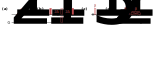
\includegraphics[]{pureshift/elements.png}%
    {\phantomsubcaption\label{fig:pureshift_elements_zs}}%
    {\phantomsubcaption\label{fig:pureshift_elements_bird}}%
    {\phantomsubcaption\label{fig:pureshift_elements_tr}}%
    {\phantomsubcaption\label{fig:pureshift_elements_psyche}}%
    \caption[Pure shift elements]{
        A selection of pure shift elements.
        \textbf{(\subref*{fig:pureshift_elements_zs})} Zangger--Sterk PSE\autocite{Zangger1997JMR}, involving the combination of a selective \ang{180} refocusing pulse and a weak gradient.
        \textbf{(\subref*{fig:pureshift_elements_bird})} BIRD PSE\autocite{Garbow1982CPL,Aguilar2011ACIE}; the delay $\Delta$ is set to $1/(4 \cdot \oneJ{CH})$.
        \textbf{(\subref*{fig:pureshift_elements_tr})} Time-reversal PSE\autocite{Sorensen1985JACS}, simply consisting of a hard pulse with variable flip angle $\beta$. Multiple spectra with different values of $\beta$ must be co-added to suppress artefacts (though this suppression is not perfect, as discussed in the text).
        \textbf{(\subref*{fig:pureshift_elements_psyche})} PSYCHE PSE\autocite{Foroozandeh2014ACIE}, consisting of two saltire pulses\autocite{Foroozandeh2018CEJ,Foroozandeh2020JMR} with flip angle $\beta$, and a weak gradient.
    }
    \label{fig:pureshift_elements}
\end{figure}


\subsubsection{Zangger--Sterk}

We are finally now in a position to study individual PSEs and their mechanisms of action.
We begin with the Zangger--Sterk (ZS, or `slice-selective') PSE\autocite{Zangger1997JMR}, in which a selective refocusing pulse and a weak gradient are simultaneously applied (\cref{fig:pureshift_elements_zs}).
In practice, an rSNOB pulse\autocite{Kupce1995JMRSB} is often used as the refocusing pulse.
The effect of the gradient is to make each spin in the sample have a spatially dependent offset; therefore, in each \textit{slice} (or cross-section) of the sample, a different spin will fall within the specific bandwidth of the refocusing pulse.
This spin is refocused by the PSE and therefore becomes the active spin \textit{within that specific slice}; the bracketing pair of CTP gradients serve to destroy coherences on all the other spins which are not inverted.
Each signal of the pure shift spectrum therefore derives from a specific slice of the sample; during direct detection, all slices simultaneously contribute to the signal, thus yielding a broadband pure shift spectrum.

The sensitivity of the ZS method tends to be low (the factor $c$ tends to be on the order of $0.01$ to $0.05$), as each signal only comes from a narrow section of the sample.
Nevertheless, it still finds wide usage in pure shift applications nowadays, especially because it is compatible with the real-time acquisition mode\autocite{Meyer2013ACIE}: as long as the pulse and the weak gradient are the same each time, then the same active spins will always be chosen in the same slice (as long as diffusion effects are ignored).
The PSE can also be customised through the bandwidth of the refocusing pulse: decreasing this improves the spatial differentiation between spins which have similar intrinsic offsets, yielding better decoupling quality, albeit at the cost of sensitivity.
The ZS element can be easily---and has been---adapted for use in many experiments, including (but not limited to) absorption-mode 2DJ spectroscopy\autocite{Pell2007JMR} and selective refocusing (SERF) experiments for the measurement of $\nJ{HH}$\autocite{Giraud2010ACIE,Gubensak2014CC,Mishra2017JMR,Buchberger2018MRC}.


\subsubsection{BIRD}

Next up is the \textit{bilinear rotation decoupling} (BIRD) pulse element (\cref{fig:pureshift_elements_bird}).
BIRD is not spatially selective like the ZS method; instead, it is \textit{isotope-selective} in that it acts as a \angang{180}{y} pulse on \carbon{}--bound protons, and does not affect \carbont{}--bound protons.
Consequently, all \carbon{}--bound protons become the active spins in the context of pure shift NMR.
The first report of the BIRD element\autocite{Garbow1982CPL}, in 1982, was clearly ahead of its time: it reported the use of an interferogram-type approach to obtain 1D pure shift spectra.
However, in the subsequent decades, this seemed to have been forgotten: BIRD found much more use as an isotope-selective rotation element in heteronuclear NMR\autocite{Uhrin1993JMRSA}, until its use as a pure shift element was `rediscovered'\autocite{Sakhaii2009JMR,Aguilar2011ACIE}.

An immediate drawback of BIRD is that it does not decouple geminal (diastereotopic) \ch{CH2} groups, as both protons would be either both active or both passive.
The sensitivity penalty of BIRD is also relatively severe: the factor $c$ derives from the natural abundance of \carbon{}, which is approximately $0.011$.
However, it is also compatible with real-time acquisition\autocite{Lupulescu2012JMR}, and has found particular success as a pure shift element in the $F_2$ dimension of HMQC and HSQC experiments\autocite{Sakhaii2009JMR,Paudel2013ACIE,Reinsperger2014JMR,Kiraly2018MRC,Nolis2019JMR_psHSQC,Singh2020JMR}: in this case, the use of BIRD leads to no loss of sensitivity as only \carbon{}--bound protons are detected in HSQC experiments anyway.%
\footnote{In fact, the sensitivity is increased by the collapse of multiplet structure.}
It should be noted that the BIRD element does not need to be combined with a hard \ang{180} pulse to form a JRE: the inverse effect of only flipping the passive spins can be accomplished by simply changing the phase of both internal \ang{180} pulses to $+y$.
Using the nomenclature of Uhr{\'i}n et al.,\autocite{Uhrin1993JMRSA} the PSE and JRE forms of the BIRD pulse can be labelled as BIRD\textsuperscript{d,X} and BIRD\textsuperscript{r,X} respectively.

\subsubsection{Time-reversal}

The \textit{time-reversal} PSE (\cref{fig:pureshift_elements_tr}) is even simpler: it consists only of one hard pulse with flip angle $\beta$\autocite{Sorensen1985JACS}.
The catch is that the experiment must be repeated with different values of $\beta$, and the results added up with specific weightings.\autocite{Griesinger1986JCP}
This leads to cancellation of \textit{some}, but not all, of the unwanted coherences: for example, on its own, it does not suppress COSY-type coherence transfer such as $I_{1-}I_{2\alpha} \to I_{1\alpha}I_{2+}$.
This proved to be inconsequential in the original application of $F_1$ decoupling in a 2D NOESY\autocite{Sorensen1985JACS}; however, it is not acceptable in a 1D context as it leads to substantial artefacts.
This will be discussed in more detail in \cref{sec:pureshift__timerev}, so a fuller analysis of the time-reversal PSE is deferred until then.


\subsubsection{PSYCHE}

Finally, we come to the PSYCHE method, which is generally considered the current state of the art for pure shift NMR.\autocite{Foroozandeh2014ACIE}
The corresponding PSE (\cref{fig:pureshift_elements_psyche}) consists of two swept-frequency pulses applied during a weak gradient: for example, a pair of chirps with opposite sweep directions can be used.
The signal-to-artefact ratio of PSYCHE can be further improved by using two \textit{saltire pulses}: these are superpositions of chirps which simultaneously sweep in both frequency directions\autocite{Foroozandeh2018CEJ}.
The operation of this PSE is not easy to fully explain\autocite{Foroozandeh2020JMR}. However, we can adopt the (not fully accurate, but still useful) instant-flip approximation\autocite{Zwahlen1997JACS,Kupce2007JMR}---that the swept-frequency pulse acts as an instantaneous \ang{180} rotation on each frequency it passes through.
Using this, the PSYCHE element (or strictly, the PSYCHE JRE, including a hard \ang{180} pulse) may be viewed as a spatially parallelised version of the anti $z$-COSY experiment\autocite{Oschkinat1986JMR,Pell2007MRC}, which we now describe.

\subsection{PSYCHE in detail}
\label{subsec:pureshift__psyche_analysis}

\begin{figure}[ht]
    \centering
    
\includegraphics[]{pureshift/psyche_detail.png}%
    {\phantomsubcaption\label{fig:psyche_detail_antizcosy}}%
    {\phantomsubcaption\label{fig:psyche_detail_cosy_suppress}}%
    {\phantomsubcaption\label{fig:psyche_detail_zqc_suppress}}%
    \caption[Detailed analysis of anti $z$-COSY and PSYCHE]{
        A closer look at the mechanism of the PSYCHE PSE.
        \textbf{(\subref*{fig:psyche_detail_antizcosy})} The $\beta$--ZQF--$\beta$ mixing period used in the original anti $z$-COSY experiment. This has a similar action to a JRE, but does not suppress COSY-type coherence transfers from spin $i$ to spin $j$.
        \textbf{(\subref*{fig:psyche_detail_cosy_suppress})} An illustration of how COSY-type artefacts are suppressed by the PSYCHE pulse element. The desired CTP which remains on spin 1 is rephased by the gradients, but the COSY CTP is dephased.
        \textbf{(\subref*{fig:psyche_detail_zqc_suppress})} An illustration of how zero-quantum terms are suppressed by the PSYCHE element through spatial averaging: in each slice of the sample (highlighted in blue and orange), the zero-quantum terms are allowed to evolve for a different duration.
    }
    \label{fig:psyche_detail}
\end{figure}

The anti $z$-COSY experiment utilises a $\beta$--zero-quantum filter (ZQF)--$\beta$ mixing period (\cref{fig:psyche_detail_antizcosy}), where $\beta$ is a small angle, typically \ang{10} to \ang{20}.
The role of the ZQF\autocite{Thrippleton2003ACIE} is to remove terms such as $I_{1-}I_{2+}$ between the two $\beta$ pulses, retaining only population terms such as $I_{1\alpha}I_{2\alpha}$.
The CTPs which this mixing period selects for ultimately give rise to peaks which lie perpendicular to the main diagonal of the spectrum.
In an elegant paper, Pell et al.\autocite{Pell2007MRC} showed that by isolating the diagonal peaks of a 2D anti $z$-COSY experiment and taking the \ang{45} projection of these, a pure shift spectrum could be obtained.
Here, we will go one step further and consider the \textit{direct} use of this element as a JRE: this will reveal some problems which are neatly taken care of by the PSYCHE experiment.

We first need to introduce how the basis operators $\{I_+, I_-, I_\alpha, I_\beta\}$ evolve under a hard pulse (applied along the $x$-axis) with flip angle $\beta$:
\begin{align}
    I_{\pm} &\xrightarrow{\beta I_x} c^2 I_{\pm} + s^2I_{\mp} \pm \frac{\mi S}{2}(I_\alpha - I_\beta) \label{eq:ipm_beta_evolution} \\
    I_{\alpha} &\xrightarrow{\beta I_x} c^2 I_{\alpha} + s^2I_{\beta} + \frac{\mi S}{2}(I_+ - I_-) \label{eq:ialpha_beta_evolution} \\
    I_{\beta} &\xrightarrow{\beta I_x} c^2 I_{\beta} + s^2I_{\alpha} - \frac{\mi S}{2}(I_+ - I_-) \label{eq:ibeta_beta_evolution}
\end{align}
where $S = \sin\beta$, $s = \sin(\beta/2)$, and $c = \cos(\beta/2)$.
Using these formulae, we can show that for a two-spin system (see Pell et al.\autocite{Pell2007MRC} for the equivalent analysis on a three-spin system), the $\beta$--ZQF--$\beta$ element converts the term $I_{1+}I_{2\alpha}$ to
\begin{equation}
    \label{eq:anti_z_cosy_transitions}
    I_{1+}I_{2\alpha} \longrightarrow
    {\underbrace{\frac{1}{2}S^2c^4 I_{1+}I_{2\beta}}_\text{term 1}}
    + {\underbrace{S^2c^2s^2I_{1+}I_{2\alpha}}_{\text{term 2}}}
    - {\underbrace{\frac{1}{4}S^2c^4I_{1\alpha}I_{2+}
    + \frac{1}{4}S^2c^4I_{1\beta}I_{2+}}_{\text{terms 3 and 4}}}
    + \cdots,
\end{equation}
where other terms with different coherence orders have been neglected (on the basis that they can be easily suppressed with bracketing CTP gradients), and terms with higher orders in $s$ have been discarded since $s = \sin(\beta/2) \ll 1$ for small $\beta$.

The first term $I_{1+}I_{2\beta}$, corresponding to the flipping of passive spins only, is the only term we want to see from a JRE.
The second term, $I_{1+}I_{2\alpha}$, corresponds to the case where neither active nor passive spins have been flipped.
In the original anti $z$-COSY work, these give rise to `off-diagonal' peaks which are part of a multiplet on the diagonal, but when projected at \ang{45} generate artefacts around the pure shift peak.
In the context of pure shift NMR, these are called `recoupling artefacts', as they arise from imperfect J-refocusing.
Note that the ratio of recoupling artefacts to desired signal is proportional to $S^2c^2s^2/S^2c^4 = \tan^2(\beta/2)$: using a smaller value for $\beta$ therefore leads to better signal-to-artefact ratios, but also lower overall sensitivity.
The PSYCHE element is similar to the $\beta$--ZQF--$\beta$ element in this regard: it does not suppress the recoupling artefacts, but instead relies on the user choosing a suitable value for $\beta$ such that the artefact-to-signal ratio is tolerably small.
If the sensitivity proves to be insufficient, the flip angle $\beta$ may be increased instead: this leads to a larger artefact-to-signal ratio, but if the sample is not concentrated anyway, it may well be that the artefacts do not rise above the noise level.%

The third and fourth terms, $I_{1\lambda}I_{2+}$ ($\lambda \in \{\alpha,\beta\}$), represent `COSY-type' coherence transfer to a coupled spin.
In the original anti $z$-COSY, these led to crosspeak multiplets at $(\Omega_1, \Omega_2)$, which could be removed by hand before taking the projection.
However, in a pure shift sequence, the peaks arising from these terms cannot simply be removed in the same way.
It is precisely this issue which precludes the $\beta$--ZQF--$\beta$ element from being directly used as a JRE, and motivates the development of the PSYCHE PSE, which \textit{does} suppress these coherence transfers.

To understand how this occurs, we invoke the instantaneous spin-flip assumption.
Each coherence $I_{i+}$ is converted (or `flipped') to a population term $I_{1\lambda}$ at a specific point $\alpha\taup$ after the start of the first chirp, and can be reconverted to a coherence on the same spin $I_{i-}$ at a time $\alpha\taup$ before the end of the second chirp (the blue CTP in \cref{fig:psyche_detail_cosy_suppress}).%
\footnote{Note the change in the sign of the coherence, which differs from the analysis of the anti $z$-COSY experiment. This arises because we are only considering the PSYCHE PSE on its own, \textit{not} the JRE.}
Here, $\taup$ is the duration of the chirp, and $0 < \alpha < 1$.
In this case, the coherence is perfectly rephased by the weak gradient applied during the chirp pulses, since the \textit{time} it experiences these gradients for is the same on both sides of the chirps.
Now, if the $I_{i+}$ term is instead converted to a coherence on a different spin $I_{j-}$, it experiences the gradient for a total duration of $\alpha\taup$ after the start of the first chirp, and also $\alpha'\taup$ before the end of the second chirp (the orange CTP in \cref{fig:psyche_detail_cosy_suppress}).
In general, $\alpha \neq \alpha'$ as spins $i$ and $j$ have different offsets; therefore, this CTP is dephased by the gradients, resulting in suppression of the COSY-type artefacts in the spectrum.

It remains to also consider how the PSYCHE element selects for the population terms between the two spin flips.
Any terms with nonzero coherence order are of course simply dephased by the weak gradient.
However, zero-quantum terms (in homonuclear systems) are not dephased by gradients, and to eliminate them in a single-scan manner, they must be spatially averaged, for example by a ZQF.
It turns out that the PSYCHE element also results in a similar spatial averaging.
Following on from the previous paragraph, the time \textit{between} the spin flips (for the desired pathways, i.e.\ not COSY-type coherence transfer) is given by $2(1 - \alpha)\taup$.
At the same time, the weak gradient induces a range of offsets across the sample, much like in the Zangger--Sterk experiment.
Thus, the offset, and thus the value of $\alpha$, for a given spin depends on which slice it is in; for example, \cref{fig:psyche_detail_zqc_suppress} uses values of $\alpha_1$ and $\alpha_2$ for two different slices (blue and orange).
If zero-quantum terms are present between the spin flips, they evolve during this time and accrue a spatially-dependent phase: summation of these during FID acquisition leads to a cancellation of these terms.
Only population terms such as $I_{1\alpha}I_{2\alpha}$ survive during this, as they do not precess during this time.

The sensitivity of PSYCHE is significantly better than for other methods: depending on the flip angle $\beta$ chosen, $c$ is typically on the order of $0.05$--$0.15$ (see also \cref{fig:fa_dependence_124} for explicit simulations).
Furthermore, it is generally more robust with respect to strong coupling compared to other pure shift methods (artefacts from strong coupling often arise due to unexpected coherence transfer\autocite{Thrippleton2005JMR}, which is suppressed in a similar way to the COSY-type artefacts).
These two factors alone have meant that PSYCHE has enjoyed substantial adoption since its introduction: a large number of 2D experiments utilising PSYCHE decoupling in either $F_1$ or $F_2$ have been developed,\autocite{Foroozandeh2014JACS,Timari2015CEJ,Koos2016ACIE,Sinnaeve2016ACIE,Aguilar2018MRC,Kaltschnee2016JMR,Ilgen2021JMR} notably the PSYCHE-iDOSY diffusion experiment\autocite{Foroozandeh2016ACIE}, where the increased resolution provided by pure shift spectroscopy translates into increased resolution in the \textit{diffusion} dimension as well.
Like the ZS element before it, the PSYCHE element has also been used for the acquisition of absorption-mode 2DJ spectra.\autocite{Foroozandeh2015CC}

Despite this success, PSYCHE suffers from one significant drawback: it cannot be used in a real-time fashion.
The PSYCHE PSE is often said to select active and passive spins in a `statistical' manner: this is because of the $c^2$ and $s^2$ terms arising from the low-flip angle pulses.
What this really means is that we do not care \textit{exactly} which spins are active and which are passive, but that a certain proportion of the spins are active and passive.
Repeated application of the PSE therefore does not select for the same active spins each time, which precludes its application to real-time acquisition.

Although the PSYCHE PSE may appear deceptively simple at first glance, the closer analysis given here (and elsewhere\autocite{Foroozandeh2018CEJ}) clearly shows that its inner workings are anything but.
Along with other ingenious experiments such as the ZQF\autocite{Thrippleton2005JMR}, ultrafast NMR\autocite{Frydman2002PNASUSA,Pelupessy2003JACS,Frydman2003JACS}, and more recently GEMSTONE\autocite{Kiraly2021ACIE}, PSYCHE is a prime example of how \textit{spatiotemporal averaging} and pulsed field gradients can be used to great effect in modern NMR spectroscopy.\autocite{Dumez2018PNMRS}

At the same time, PSYCHE itself is not \textit{perfect}: it does not fully suppress recoupling artefacts, and can only be used in the interferogram mode.
To improve on PSYCHE would therefore entail one of the following:
\begin{enumerate}
    \item increasing the sensitivity (while maintaining purity);
    \item increasing the purity (while maintaining sensitivity); or
    \item developing a pure shift element which is compatible with real-time acquisition while giving comparable sensitivity and purity to PSYCHE.
\end{enumerate}

The sections which follow describe my efforts towards objectives (1) and (2).

